\section{Background Research \& Analysis}

\subsection{Application Research \& Analysis}
This section details the research behind the data used in Opticaff, including the data source, calendar data and the caffeine calculations that will be used in the prototype. 

\subsubsection{Data Source}
\label{sec:Data}
OptiCaff used the Open Data Service from the University of Southampton \cite{DataSouthampton} to retrieve the relevant information for the application. This service provides open linked data about some of the administrative information regarding the university. It also provides a SPARQL Endpoint \cite{SotonSparql} (a service which facilitates users querying a knowledge base using the SPARQL query language) \cite{SparqlEndpoint}. OptiCaff utilises this with a few specialist queries, and combined with user preferences can provide the user with a wide selection of caffeine choices around campus. 

\subsubsection{Calendar Research \& Analysis}
\label{sec:calendar}
OptiCaff’s objectives include the use of university timetables to schedule caffeine level notifications. 
Sussed is Southampton university’s student portal that displays a student’s timetable, OptiCaff will need to access the timetable through Sussed. 
This is currently the only way to obtain a student's timetable given that its not freely available as open data. 
Another Southampton university produced application, iSoton, has been able to do this process showing that it is possible.
Further investigation however has shown that this is not a trivial process.

An alternative solution is to use Google Calendar which can be easily integrated into Android given that they are both Google Products \cite{calendar}.
This has the disadvantage however that it requires the user to either have or set up a Google Calendar detailing their timetable information. 
 
Overall given the prototype nature of this application and ability to use Google Calendar in a much simpler fashion it was decided that Opticaff would use Google Calendar. 

\subsubsection{Caffeine Research \& Analysis} 
\label{sec:Caffeine}
In order to provide the caffeine management element of this application, the different levels of caffeine that appeared in beverages and its affect on human beings needed to be researched. This section details the caffeine levels and decay rate that has been used in Opticaff. 

\underline{Caffeine Levels in Products} \newline
Given the vast range of different cafffeinated products and the limited time to produce a prototype application, it was decided that the products displayed by OptiCaff would be grouped into four different types of drink, and each type would be allocated an average caffeine content. Below is a table showing these totals, which were obtained these sources \cite{Coke} \cite{TeaCoffee} \cite{EnergyDrink}.

\begin{center}
\begin{tabular}{|l|l|}
\hline
\textbf{Drink Category} & \textbf{Average Caffeine Content (mg)} \\\hline
Tea & 40 \\\hline
Coffee & 54 \\\hline
Energy Drinks & 80 \\\hline
Soft Drinks & 34.5 \\\hline
\end{tabular}
\end{center}

\underline{Caffeine Decay Levels} \newline
In addition to calculating the level of caffeine obtained from a specific product, it was also important to work out the optimum caffeine levels and how long it would take the caffeine to ``decay" within the body so that the next dosage time could be predicted. For the purposes of the prototype, Opticaff uses the same optimum caffeine levels as it's competitor Caffeine Zone 2 (detailed in Section \ref{sec:competitors}) uses which are between 200 and 400mg \cite{CaffeineZoneInfo}. The half life of caffeine ranges between 2.5 and 4.5 hours \cite{CaffeinePharmacology} \cite{CaffeinePharmacy} and to simplify matters 4 was chosen as the number to use in Opticaff and was calculated using the half life formula detailed here: \cite{HalfLife}.
 
\subsection{Market Research \& Analysis}
This section details the market research analysed for Opticaff.
The Coffee market was researched as were the different mobile development platforms; which were analysed to determine the most suitable one to use for this prototype application. 
Finally the potential competitors to Opticaff were detailed and analysed to see if any of them pose a genuine threat against it. 

\subsubsection{Coffee Research \& Analysis}
Coffee consumption in the United Kingdom has steadily increased over the past decade. 
In particular the past five years been seen an explosive increase, there are several theories as to why this is the case.
Firstly, instant coffee shops have become more common on our high streets. 
Companies such as Starbucks\texttrademark and Costa\texttrademark have been opening more stores as more citizens have been buying instant coffee; this doesn’t show any signs of slowing down either as Starbucks have recently announced 300 new stores to be opened over the next five years \cite{starbucks}.

Secondly, these brands have contributed to the newfound ‘coolness’ that is associated with coffee \cite{popular}. 
Lastly, there is evidence that the economic climate has played a part in coffee’s rise. 
Also known as the ‘lipstick effect’, Britons have been unable to afford expensive treats for themselves so they have been spending on cheaper treats, a good example of which is coffee \cite{costa}.
This research is important to OptiCaff because it shows that the coffee industry is on the rise, and it would not make business sense for us to invest in a declining industry.

\begin{figure}[ht]
\begin{center}
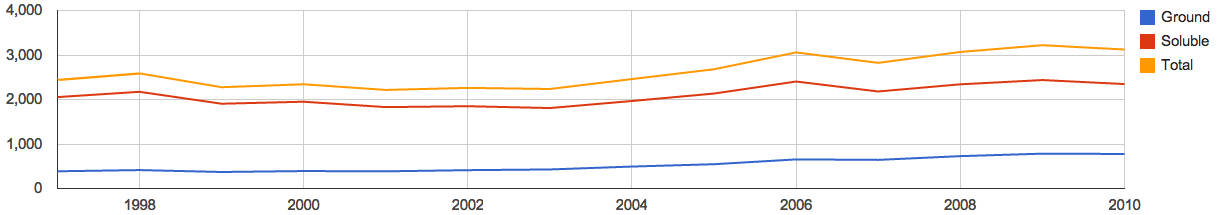
\includegraphics[trim = 0mm 0mm 0mm 0mm, clip, scale=0.6]{images/CaffeineGraph.png}
\caption{Coffee Statistics 2010 \cite{CoffeeStats}} 
\end{center}
\end{figure}

\subsubsection{Mobile Platform Research}
\label{sec:Mobile}
OptiCaff ’s purpose lent itself heavily to being a mobile application, and as such that sparked the debate of what platform it should be developed for. 
There are various mobile operating systems that Opticaff could be deployed on \cite{differentOS}:

\begin{itemize}
	\item{Google's Android}
	\item{Apple's iOS}
	\item{Blackberry's RIM}
	\item{Windows Mobile}
\end{itemize}

Based on the Smartphone Operating System statistics from June 2011 Android and Apple are dominating the market at present. 
Therefore these were the two platforms that were considered.

\begin{figure}[ht]
\begin{center}
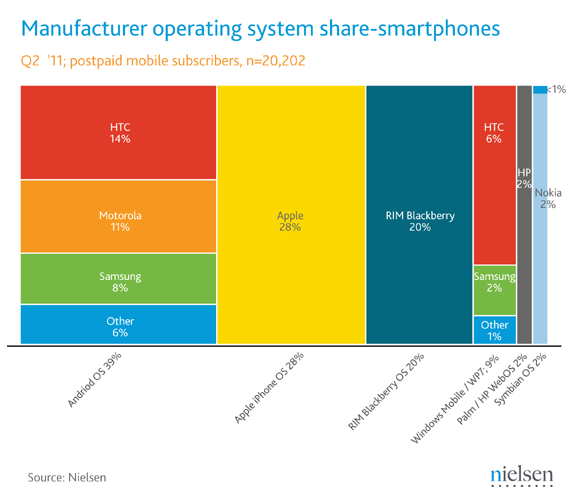
\includegraphics[trim = 0mm 0mm 0mm 0mm, clip, scale=0.6]{images/smartphone.png}
\caption{Manafacture Operating system share-smartphones June 2011 \cite{smartphone}}
\end{center}
\end{figure}

The following elements were considered in regards to which platform to use: language, development requirements and popularity of the apps for that operating system.

\underline{Programming Language}
\begin{itemize}
	\item{iOS requires applications to be written in Objective C \cite{objectivec}.}
	\item{The Android Operating System requires applications to be written in Java \cite{AndroidSDK}.}
\end{itemize}

\underline{Development Requirements}
\begin{itemize}
	\item{The only IDE available for developing iPhone applications is Xcode and there is a requirement to have Apple's iOS SDK installed \cite{iOS}. Both of these are only available to OS X users and therefore Apple Computers.}
	\item{Android doesn't require any special hardware to develop an application. The Android SDK is freely available and it's recommended development enviroment Eclipse \cite{Eclipse} is also free.}
\end{itemize}

\underline{Application Popularity}
\begin{itemize}
	\item{Apple's App Store is currently the more popular at 25 billion downloads \cite{AppleDownload}}
	\item{Google Play (Android's market place) was reported to have reached 10 billion downloads in December 2011 \cite{AndroidDownload}}
\end{itemize}

It was decided that for the prototype application, Android would be the simpler option for the following reasons:
\begin{itemize}
	\item{Android uses Java. All members of the team are experienced in Java development one member has experience in Android Development.}
	\item{Android can be developed on any platform which is useful as the group uses a combination of OSX, Linux and Windows.}
	\item{Google Play may be less popular than Apple's app store, however it still holds a large user base and it was decided that ease of development was a higher priority for a prototype application.}
\end{itemize}

\subsubsection{Gamification Research \& Analysis}
A common issue for new apps is user retention; a method of increasing this is Gamification \cite{gamification1}. Gamification is the practise of adding game-like elements to something that is not already a game, e.g. a to-do list \cite{gamification2}. There are ways in which gamification can be applied to OptiCaff.

\begin{enumerate}
	\item{Use of achievements or awards. Achievements are used to recognise when a player has fulfilled certain conditions when playing a game. An example of how this could be used with OptiCaff would be giving an achievement to a user that has stayed in the optimum caffeine range for 3 hours.}
	\item{Use of leaderboards. A leaderboard would show the users that are the best at using OptiCaff in a specified way, an example of this would be show the users that stay in the optimum range for the longest time.}
\end{enumerate}

Based on this research, it was decided that OptiCaff would use leaderboards as a method of gamification, provided that it is done in a safe way. 
This is because leaderboards can link all of the users of OptiCaff turning it into a multiplayer game. 
Obviously as with any game there would be the potential to cheat by pressing the button without actually consuming the caffeine, but this still doesn't detract from the fun element. 
One of the dangers of gamification is extreme behaviour, OptiCaff will not reward behaviour that is potentially dangerous, e.g. rewarding the user that has the highest caffeine intake.

\subsubsection{Monetisation Research \& Analysis}
It is more challenging to make money from Android Applications as opposed to Apple iOS Applications according to a report from Distimo, an app store analysis company \cite{monetisiation}. 
The report suggests several methods to maximise the money earned, these assume that the app is high enough quality to be sold.

\begin{enumerate}
	\item{80\% of paid applications have been bought less than 100 times.}
	\item{In-app advertising can either make a lot of money or very little, it depends on the amount of users an app has.}
	\item{Finally, it is common on app stores/marketplaces to have a paid version of an app that is also free. There is no difference in the function of the app, though a paid version would not display advertisements. This would give the user the choice to use the OptiCaff free or paid version though there would be income for the team either way.}
\end{enumerate}

Based upon these three points it has been decided that OptiCaff would be developed as a free and paid version that contains advertising in the free version.
The next logical step after gaining a significant user base would be to pitch the application to the owners of the caffeine vendors for funding in exchange for favouring their points of service within the application.  

\subsubsection{Competitors Research \& Analysis}
\label{sec:competitors}
This section details both the direct and indirect competitors to Opticaff and ascertains if any of them pose a substantial threat. 

Caffeine Finder is a BlackBerry application that offers some of the same functionality that OptiCaff will provide; this makes Caffeine Finder a direct competitor of OptiCaff. 
Caffeine Finder directs a user to the nearest restaurant or café, give the address and even display reviews of the destination if available. 
There are however several negative points regarding this application:
\begin{itemize}
	\item{The chosen platform was the BlackBerry which has a small screen compared to Android phones and iPhones.} 
	\item{The application doesn’t inform the user when the optimum time to have a coffee or other caffeinated drink is.}
	\item{A user may already be tired before they think to check Caffeine Finder which is something OptiCaff will try and prevent.} 
	\item{The application was released in 2005 and has not been updated regularly since that time, this is shown by reports that it is not fully compatible with newer operating systems.}
\end{itemize}

Caffeine Zone 2 Lite is a free iPhone application that tracks the amount of caffeine in the body, OptiCaff will also have caffeine tracking ability and alerts. 
This makes Caffeine Zone 2 Lite a direct competitor, although OptiCaff offers a superior service for the following reasons:  
\begin{itemize}
	\item{OptiCaff offers a complete solution, Caffeine Zone 2 Lite only tells the user when they should have caffeine, it makes no effort to tell the user where they can get a caffeinated drink.} 
	\item{The alerts generated do not consider the user’s schedule, OptiCaff will look at the user’s calendar to see if they require an earlier warning for caffeine so as to accomodate their schedule.}
	\item{Caffeine Zone 2 Lite is focussed on being an educational tool about caffeine use this is in contrast to OptiCaff which will prioritise providing a service.}
\end{itemize}

One of the issues of using open data is that the data itself can be considered an indirect competitor of OptiCaff. It could be possible for another product to be created that uses the same data set, this means that OptiCaff could have more potential competitors than it would if it used closed data. OptiCaff could not be replicated by a competitor only using the same open data however, this is because there will be caffeine level prediction and notification features implemented.
 
Table 2 summarises the competative edge of Opticaff, illustrating how it combines the key features of its competitors into a superior all encompassing service:

\begin{table}[ht]
\caption{Table of Opticaff's Competitors}
\begin{tabular}{|p{210pt}| p{50pt} | p{46pt} | p{46pt} | p{46pt} |}
    \hline
     	& 
	Caffeine Finder & 
	Caffeine Zone & 
	Caffeine Data & 
	Opticaff
\\ \hline
   	Does this app allow you to locate caffeine sources? & 
	\huge{\textcolor{green}{\Pisymbol {pzd} {52}}} & 
	\huge{\textcolor{red}{\Pisymbol {pzd} {56}}} &
	\huge{\textcolor{green}{\Pisymbol {pzd} {52}}} & 
	\huge{\textcolor{green}{\Pisymbol {pzd} {52}}}
\\ \hline
    	Does this app direct you to caffeine sources? & 
	\huge{\textcolor{green}{\Pisymbol {pzd} {52}}} & 
	\huge{\textcolor{red}{\Pisymbol {pzd} {56}}} &
	\huge{\textcolor{red}{\Pisymbol {pzd} {56}}} &
	\huge{\textcolor{green}{\Pisymbol {pzd} {52}}}
\\ \hline
    	Does this app help you to manage caffeine content? & 
	\huge{\textcolor{red}{\Pisymbol {pzd} {56}}} & 
	\huge{\textcolor{green}{\Pisymbol {pzd} {52}}} & 
	\huge{\textcolor{red}{\Pisymbol {pzd} {56}}} &
 	\huge{\textcolor{green}{\Pisymbol {pzd} {52}}}
\\ \hline
    	Does this app help you to manage caffeine content in relation to your day's activities? & 
	\huge{\textcolor{red}{\Pisymbol {pzd} {56}}} & 
	\huge{\textcolor{red}{\Pisymbol {pzd} {56}}} &
	\huge{\textcolor{red}{\Pisymbol {pzd} {56}}} &
 	\huge{\textcolor{green}{\Pisymbol {pzd} {52}}}
\\ \hline
\end{tabular}
\end{table}
